\documentclass{beamer}
\usepackage[T1]{fontenc}
\usepackage[utf8]{inputenc}
\usepackage{graphicx}
\usepackage[english]{babel}
\usetheme[
    outer/progressbar=foot
]{metropolis}
\usepackage{listings}
\usepackage[scaled=.8]{beramono}
\usepackage{subcaption}
\usepackage{booktabs}

\title{Approximative Linear $t$-SNE Using $k$-Means}
\date{\today}
\author{Sonja Biedermann, BSc}
\institute{Fakultät für Informatik\\Universität Wien}
\titlegraphic{\hfill
\includegraphics[height=1cm]{logo}}

\definecolor{asparagus}{rgb}{0.53, 0.66, 0.42}
\definecolor{alizarin}{rgb}{0.82, 0.1, 0.26}
\definecolor{chromeyellow}{rgb}{1.0, 0.77, 0.05}
\definecolor{chromeyellow}{rgb}{1.0, 0.65, 0.0}

\lstset{commentstyle=\color{darkgray},postbreak=\space,breakindent=5pt,breaklines,basicstyle=\ttfamily\footnotesize,label=DescriptiveLabel}

\makeatletter
\def\lst@MSkipToFirst{%
    \global\advance\lst@lineno\@ne
    \ifnum \lst@lineno=\lst@firstline
        \def\lst@next{\lst@LeaveMode \global\lst@newlines\z@
        \lst@OnceAtEOL \global\let\lst@OnceAtEOL\@empty
        \ifnum \c@lstnumber>0
            \vspace{2 mm}
        \fi
        \lst@InitLstNumber % Added to work with modified \lsthk@PreInit.
        \lsthk@InitVarsBOL
        \c@lstnumber=\numexpr-1+\lst@lineno % this enforces the displayed line numbers to always be the input line numbers
        \lst@BOLGobble}%
        \expandafter\lst@next
    \fi}
\makeatother

\definecolor{BlueTOL}{HTML}{0064a7}
\definecolor{BrownTOL}{HTML}{666633}
\definecolor{GreenTOL}{HTML}{225522}
% \setbeamercolor{normal text}{fg=BlueTOL,bg=white}

\definecolor{Purple}{HTML}{911146}
\definecolor{Orange}{HTML}{CF4A30}
\definecolor{Blue}{HTML}{0066a1}
\definecolor{DarkBlue}{HTML}{00466f}

% \setbeamercolor{alerted text}{fg=Orange}
% \setbeamercolor{frametitle}{bg=Purple}

\begin{document}
\maketitle

\begin{frame}{Agenda}
    \setbeamertemplate{section in toc}[sections numbered]
    \setcounter{tocdepth}{1}
    \tableofcontents
\end{frame}

\section{Introduction}

\begin{frame}[fragile]{Introduction}
\end{frame}

\section{$t$-SNE And Its Variants}

\subsection{Introduction}

\begin{frame}[fragile]{SNE}
    \begin{itemize}
        \item Stochastic Neighborhood Embedding: two probability distributions
            \begin{itemize}
                \item high dimensional: $p_{j | i}$, probability that $i$ picks $j$ as its neighbor
                \item low dimensional: $q_{j | i}$
            \end{itemize}
        \item optimization problem
        \item objective: Kullback-Leibler divergence
            \[
                KL(P \, || \, Q) = \sum_i \sum_j p_{ij} \log \frac{p_{ij}}{q_{ij}}
            \]
        \item intuition: neighborhood encoded as distribution
        \item find low-dimensional points whose neighborhood has similar encoding
        \item optimized by gradient descent --- difficult, not convex, many local minima
    \end{itemize}
\end{frame}

\begin{frame}[fragile]{$t$-SNE}
    \begin{itemize}
        \item qualitative issue of SNE: crowding problem
            \begin{itemize}
                \item lower dimensional space has much less volume
                \item many points moderately far away, not enough space
            \end{itemize}
        \item solution: fat-tailed distribution in low-dimensional space
    \end{itemize}

    \begin{figure}[h]
        \centering
        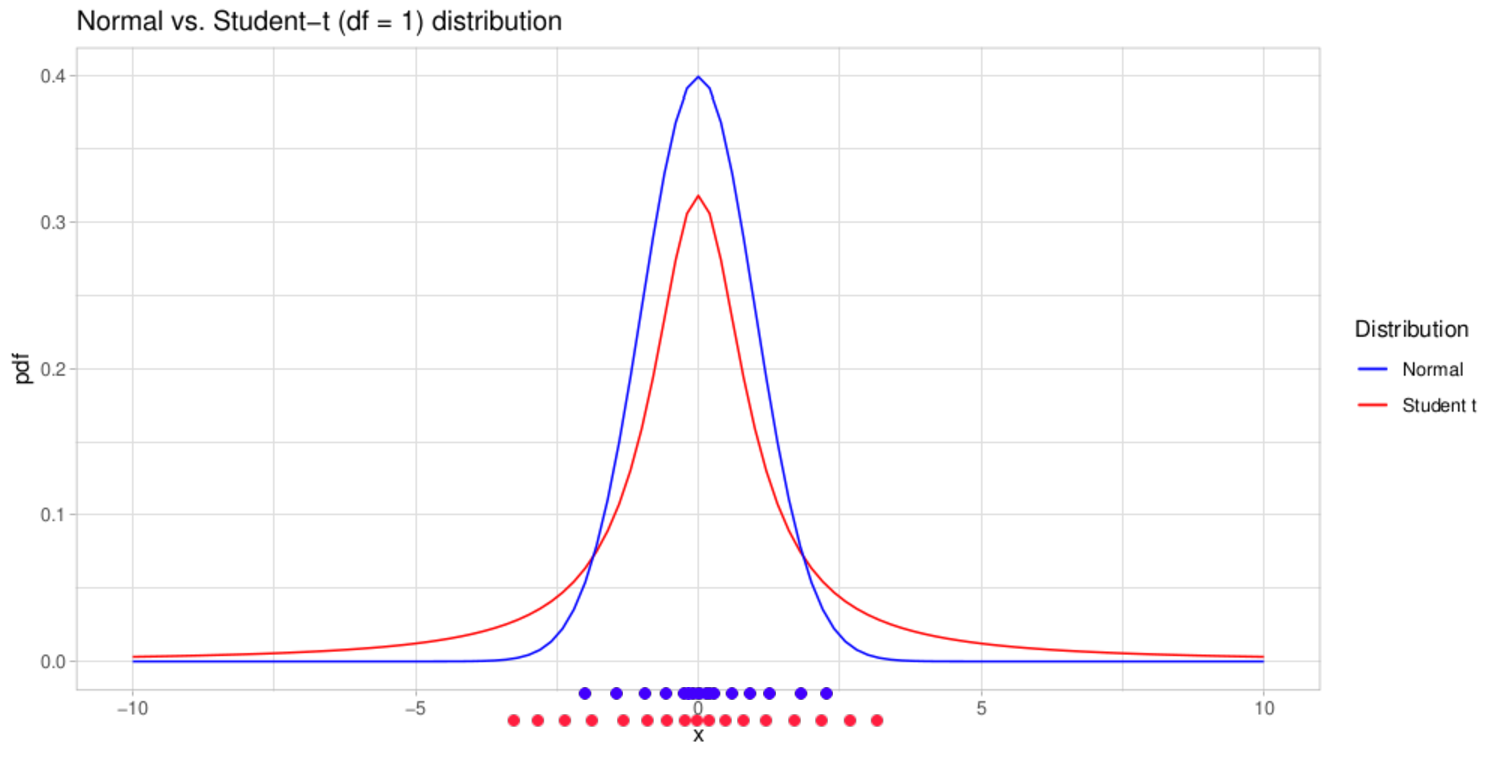
\includegraphics[height=.5\textheight]{t_vs_norm}
    \end{figure}
\end{frame}

\begin{frame}[fragile]{$t$-SNE}
    \begin{columns}
    \begin{column}{0.6\textwidth}
        \begin{itemize}
            \item popular due to visual properties
            \item problems:
                \begin{itemize}
                    \item difficult to optimize objective
                    \item computational complexity $\mathcal{O}(n^2)$
                    \item often misinterpreted
                \end{itemize}
        \end{itemize}
    \end{column}
    \begin{column}{0.38\textwidth}
        \begin{figure}[h]
            \centering
            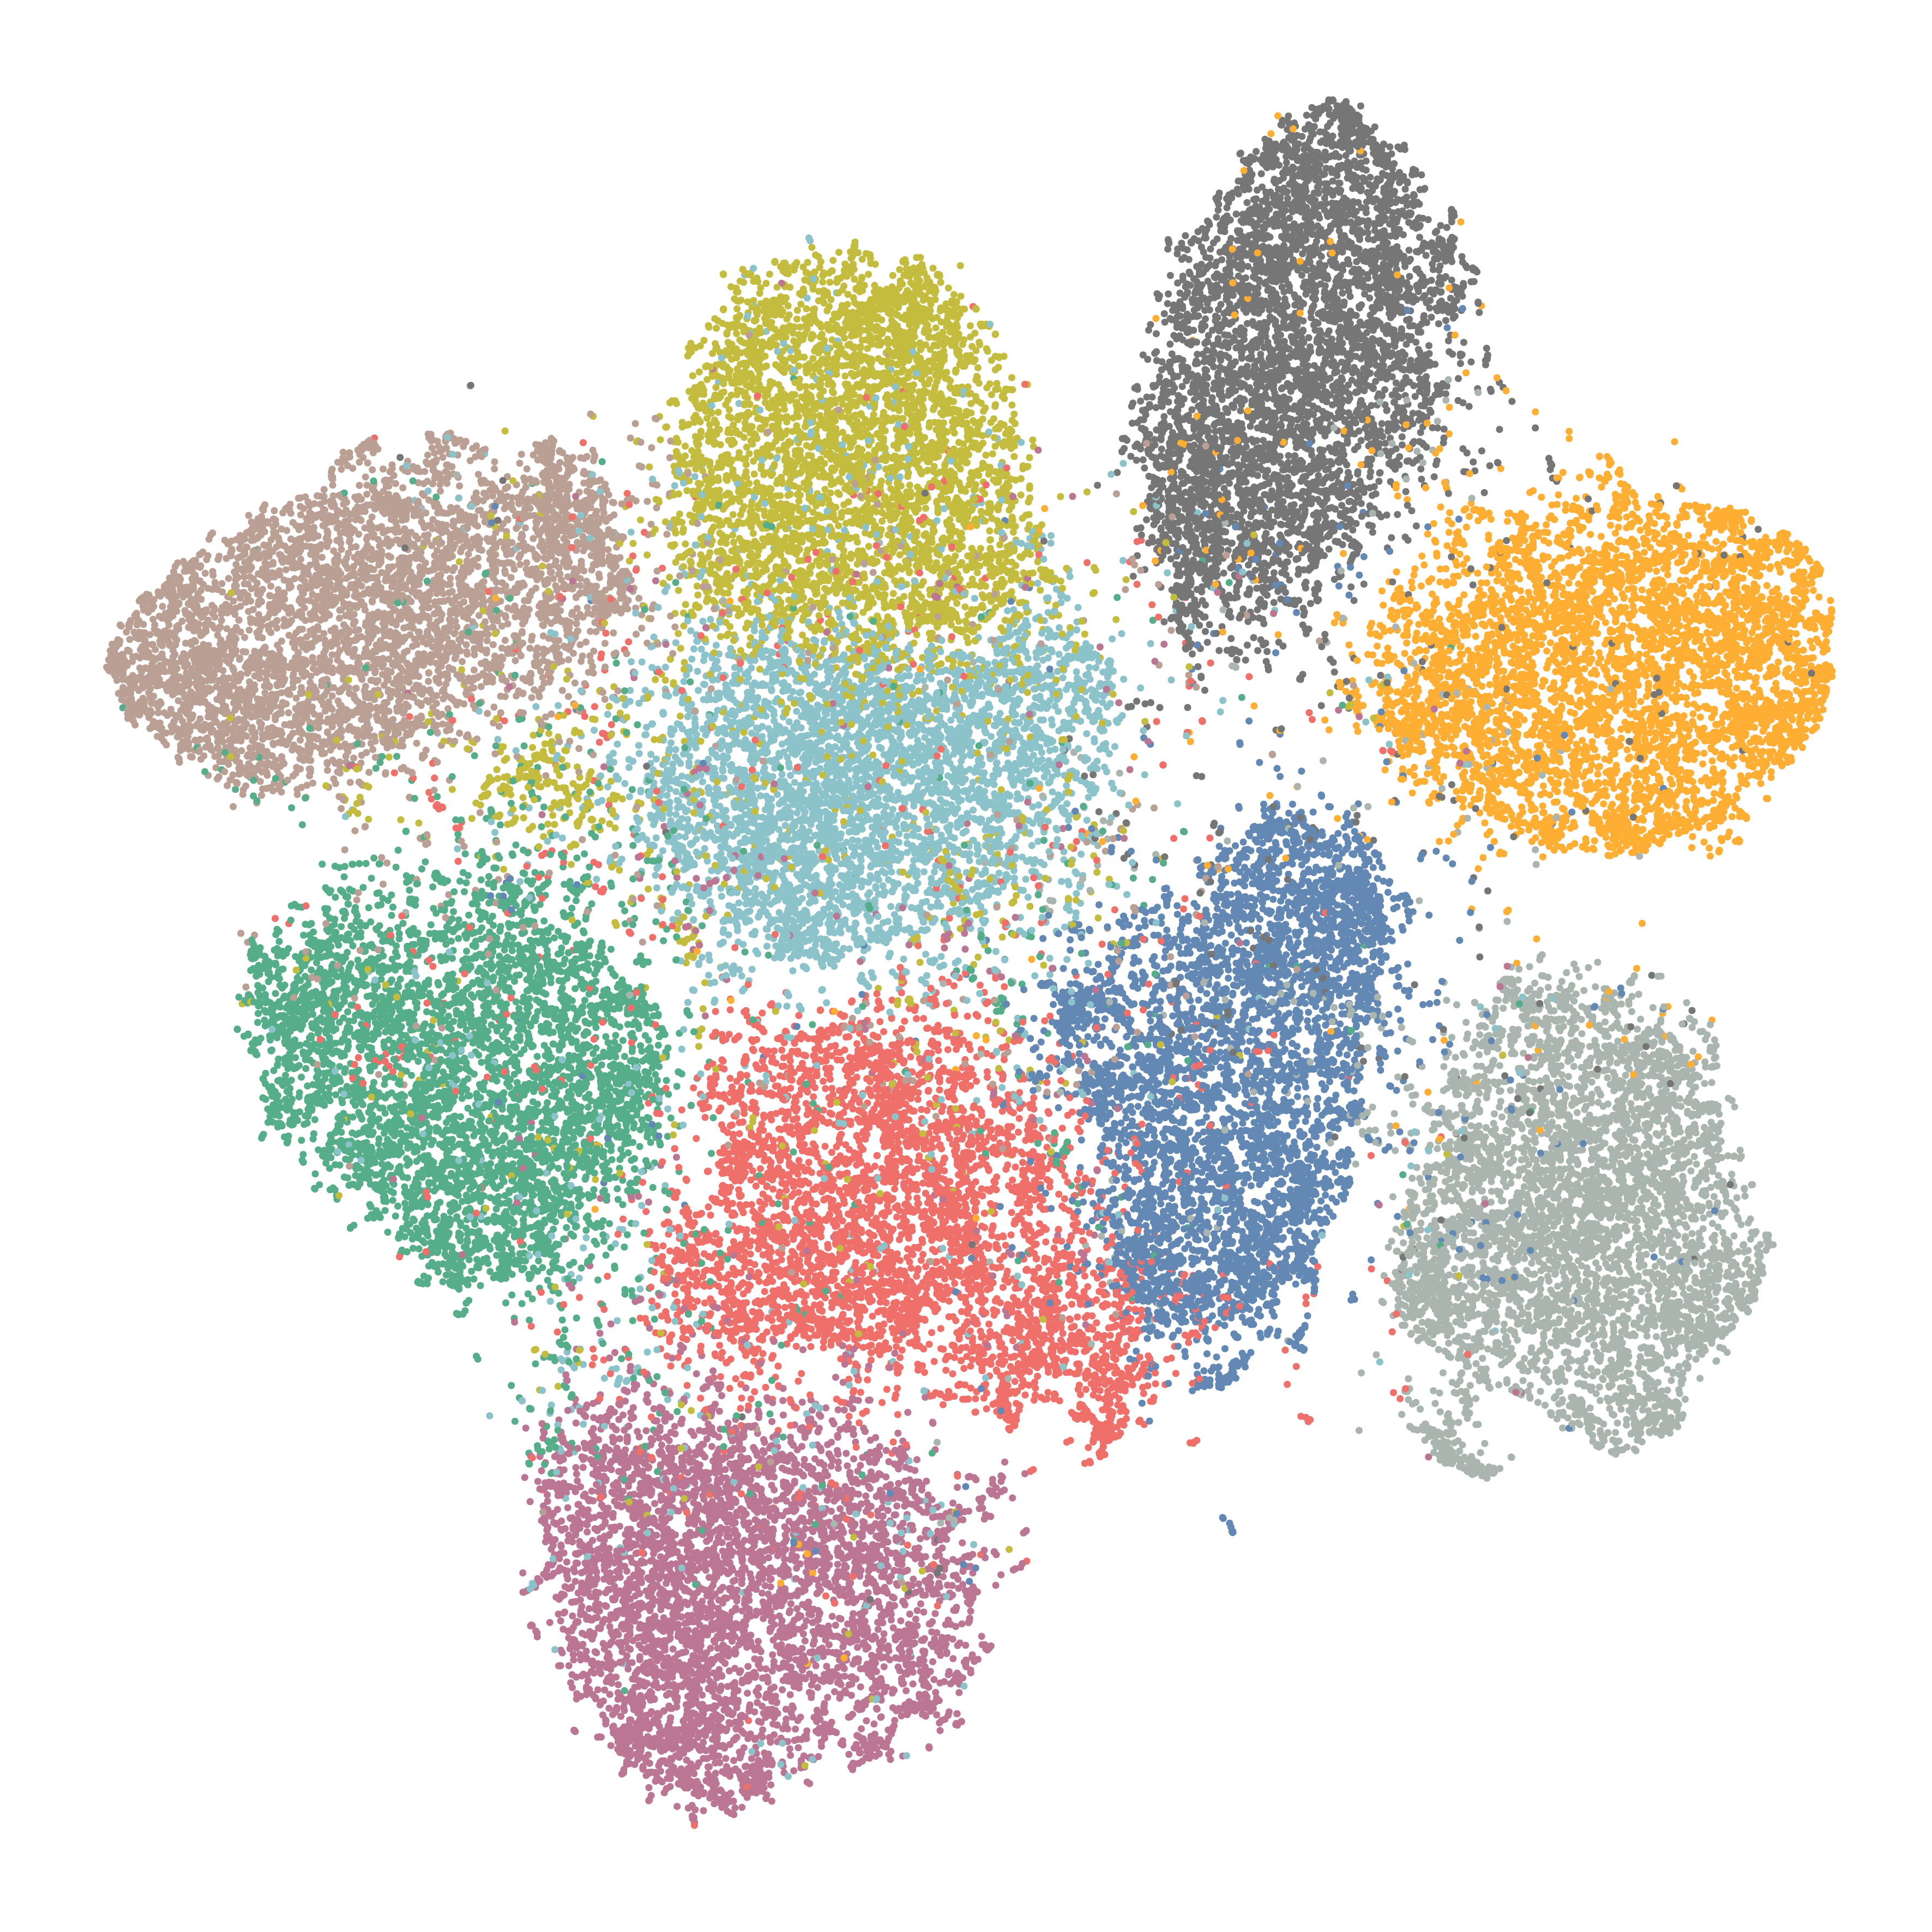
\includegraphics[width=\textwidth]{tsne_emb_cifar}
        \end{figure}
    \end{column}
\end{columns}
\end{frame}

\begin{frame}[fragile]{Related Work (Selection)}
    Barnes-Hut $t$-SNE
    \begin{itemize}
        \item use trees to
            \begin{itemize}
                \item speed up nearest neighbor search
                \item summarize points to speed up computation
            \end{itemize}
        \item computational complexity $\mathcal{O}(n \log n)$
        \item introduces quality-speed tradeoff parameter $\theta$
    \end{itemize}
\end{frame}

\begin{frame}[fragile]{Related Work (Selection)}
    FI$t$-SNE
    \begin{itemize}
        \item interpolates onto equispaced grid
        \item uses FFT to compute convolution
        \item uses random tree based library\footnote{\url{https://github.com/spotify/annoy}} to find ANNs
        \item computational complexity $\mathcal{O}(n)$
    \end{itemize}
\end{frame}

\begin{frame}[fragile]{Related Work (Selection)}
    UMAP
    \begin{itemize}
        \item another common criticism of $t$-SNE is the lack of theoretical foundation
        \item UMAP borrows from topological analysis and manifold theory to create theoretical foundation
        \item similar to $t$-SNE, but
            \begin{itemize}
                \item objective is cross entropy of two fuzzy set
                \item different kernel in high-dimensional and low-dimensional space
                \item different normalization
            \end{itemize}
        \item objective allows usage of negative sampling
        \item empirical complexity of $\mathcal{O}(n^{1.14})$ \footnote{due to NNDescent, otherwise $\mathcal{O}(n)$}
    \end{itemize}
\end{frame}

\section{Approximative Linear $t$-SNE}

\subsection{Using Approximate Nearest Neighbors}

\begin{frame}[fragile]{Using Approximative Nearest Neighbors: LSH}
    \begin{columns}
    \begin{column}{0.6\textwidth}
        \begin{itemize}
            \item ANN scheme of choice: Locality Sensitive Hashing
            \item LSH family: Cross Polytope
            \item LSH intuition: similar items should collide into the same hash bucket
            \item widely used in similarity search
        \end{itemize}
    \end{column}
    \begin{column}{0.38\textwidth}
        \begin{figure}[h]
            \centering
            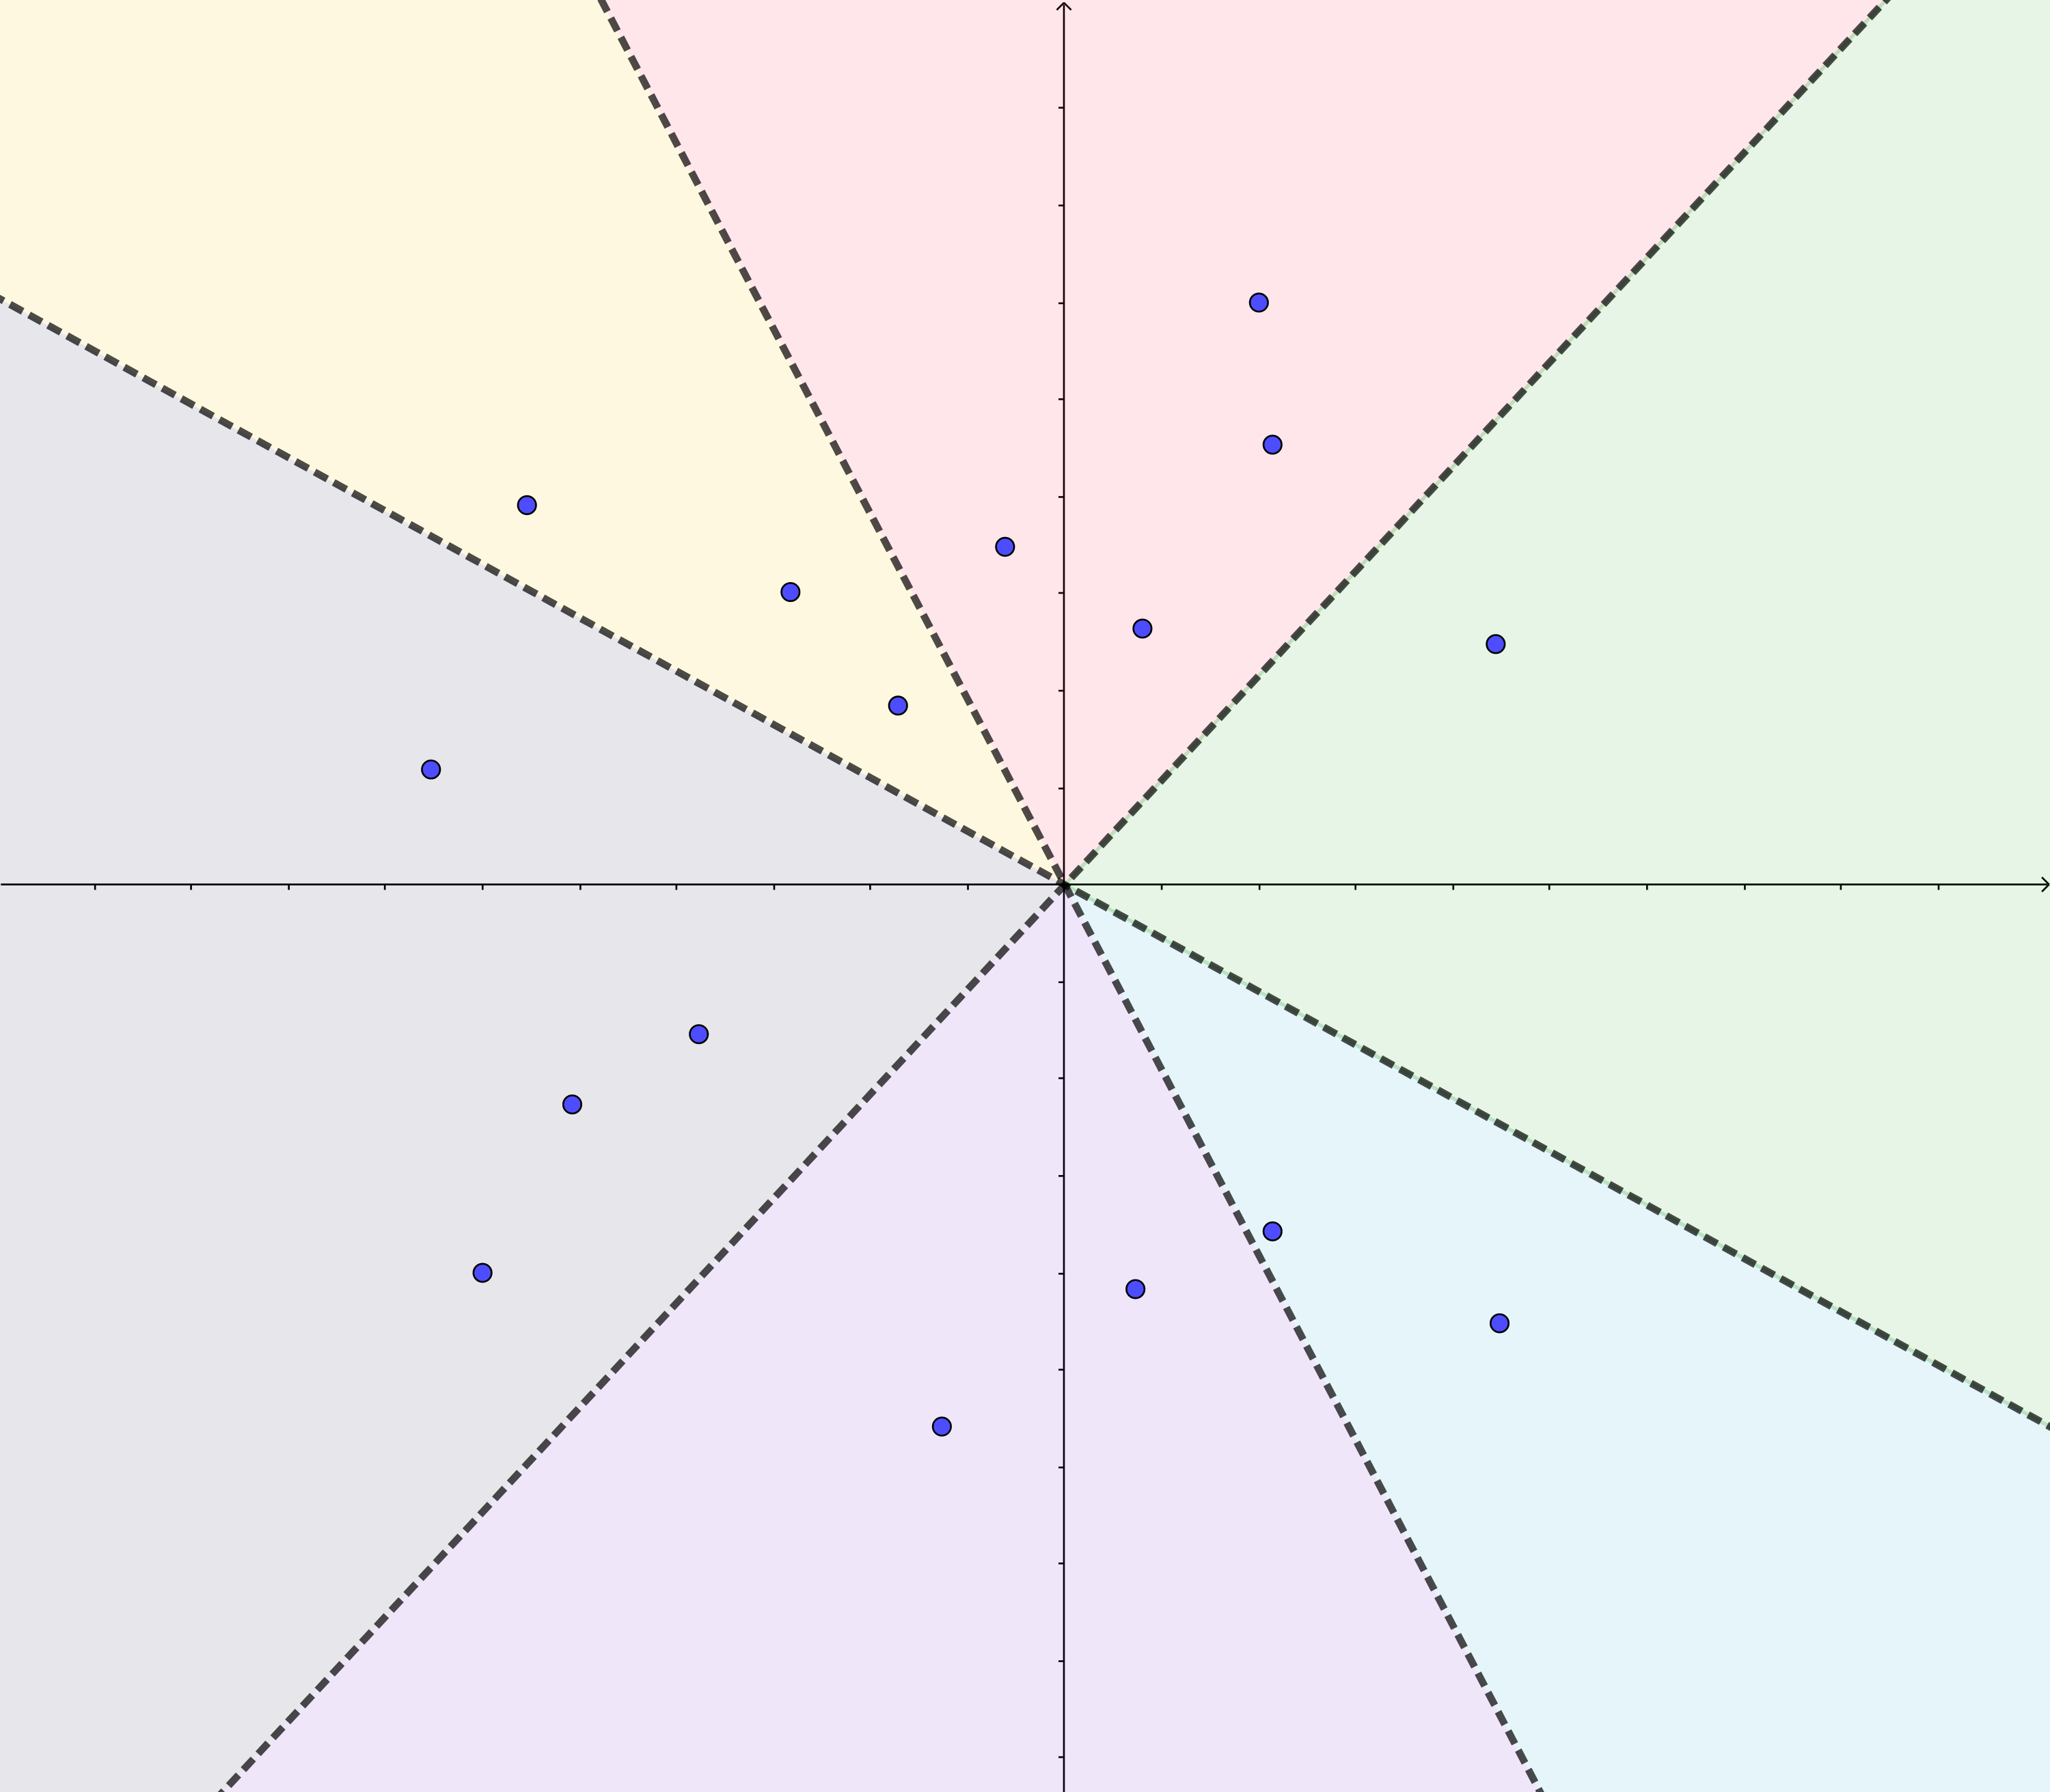
\includegraphics[width=\textwidth]{srp}
        \end{figure}
    \end{column}
\end{columns}
\end{frame}

\subsection{Using $k$-Means}

\begin{frame}[fragile]{Using $k$-Means}
    % \begin{columns}
    % \begin{column}{0.6\textwidth}
        % \begin{itemize}
            % \item summarize points by using $k$-Means to segment low-dimensional space
            % \item clustering need not be good---run for 10 iterations
            % \item cluster centers (centroids) are used to summarize
                % entire cluster
        % \end{itemize}
    % \end{column}
    % \begin{column}{0.38\textwidth}
        % \begin{figure}[h]
            % \centering
            % 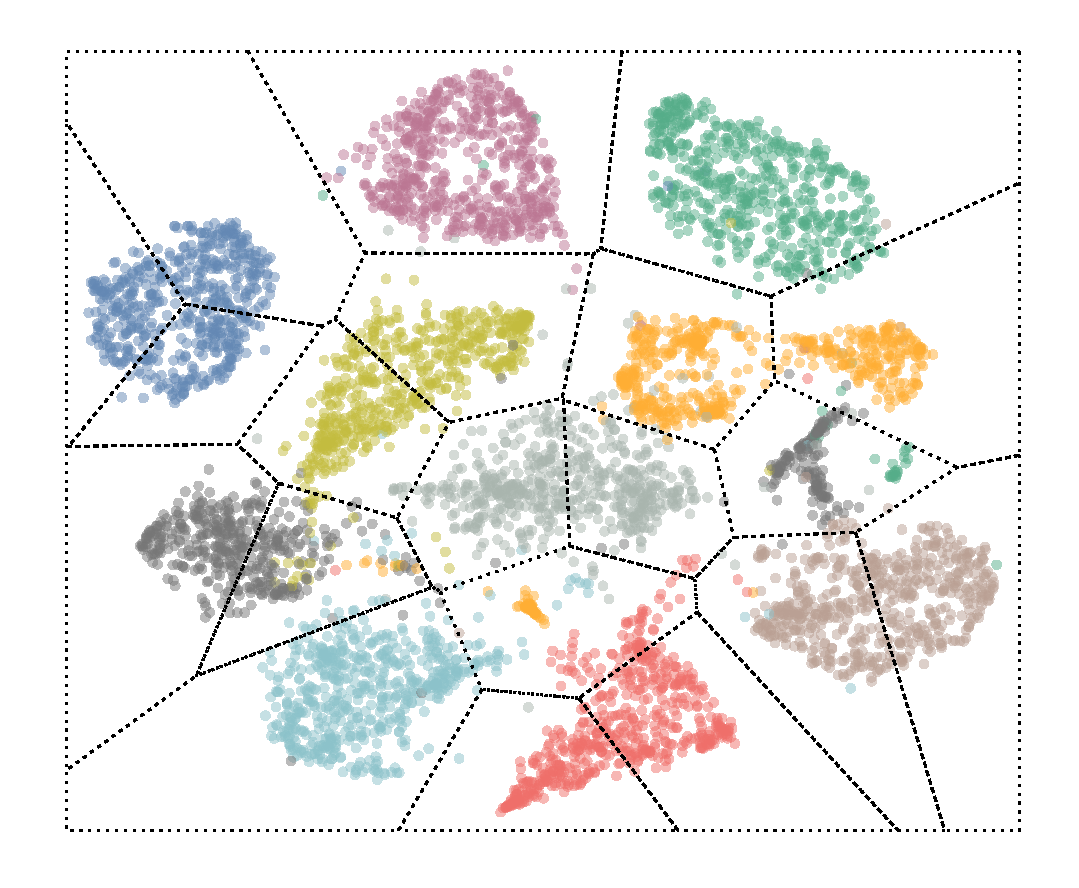
\includegraphics[width=\textwidth]{voronoi}
        % \end{figure}
    % \end{column}
% \end{columns}
        % \begin{figure}[h]
            % \centering
            % 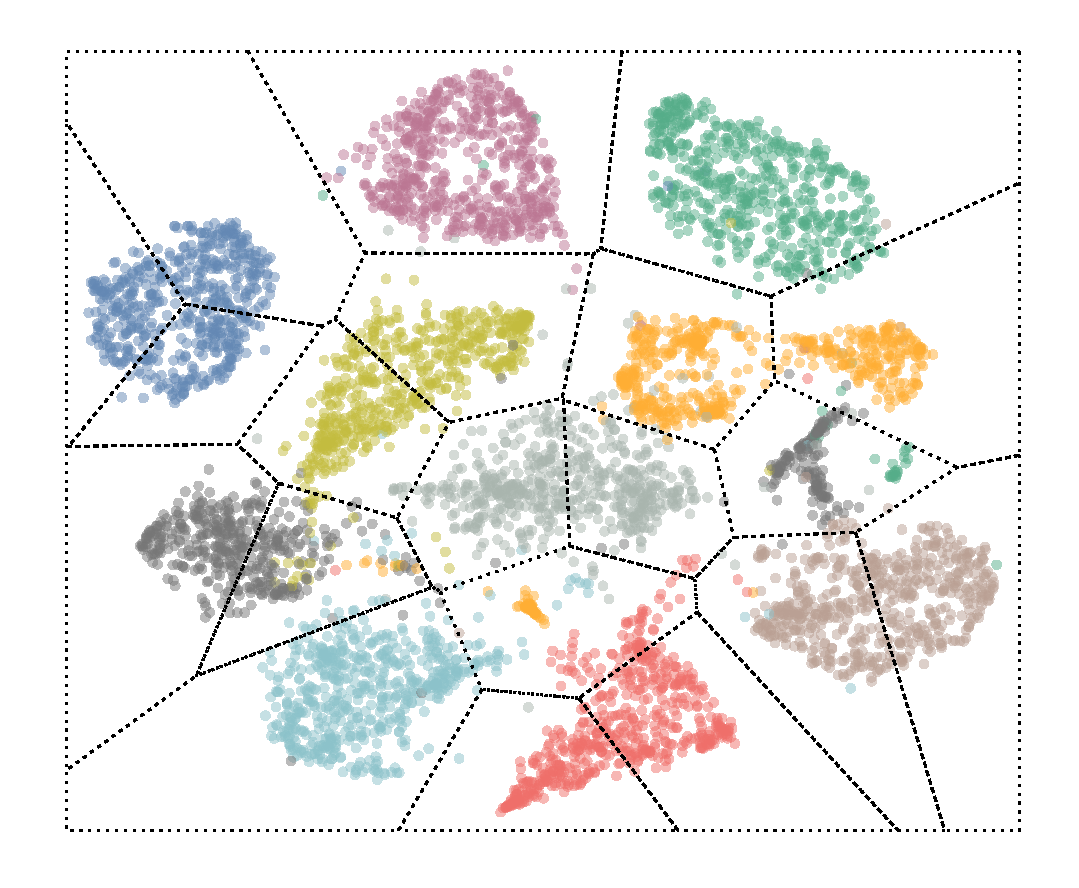
\includegraphics[width=.6\textwidth]{voronoi}
        % \end{figure}
        \begin{itemize}
            \item summarize points by using $k$-Means to segment low-dimensional space
            \item fixed $k$ (in contrast to data dependent in Barnes-Hut $t$-SNE)
            \item clustering need not be good---run for 10 iterations
            \item cluster centers (centroids) are used to summarize
                entire cluster
        \end{itemize}
\end{frame}

\begin{frame}[fragile]{Using $k$-Means}
    \begin{figure}[h]
        \centering
        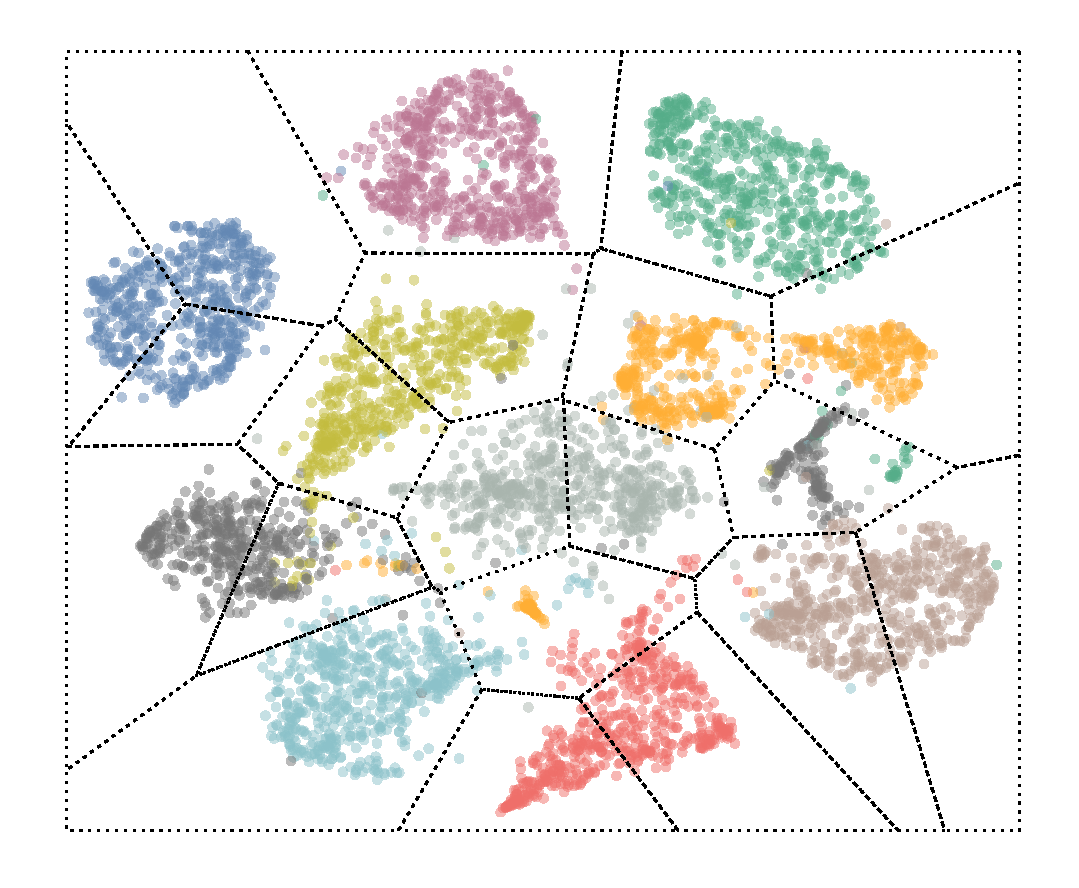
\includegraphics[width=.6\textwidth]{voronoi}
        \caption{Voronoi diagram implied by $k$-Means clustering}
    \end{figure}
\end{frame}

\begin{frame}[fragile]{Putting it all together: $t$-SNE's gradient}
    \begin{align*}
        \frac{\partial KL(P||Q)}{\partial y_i} &= \sum_{j \neq i} p_{ij}q_{ij}Z(y_i - y_j) - \sum_{j \neq i} q_{ij}^2Z(y_i - y_j) \\
        &= F_\text{attr} - F_\text{rep} \\
    \end{align*}

    \vspace{-2em}
    \quad where $Z = \sum_{k \neq l} (1 + || y_k - y_l||^2)^{-1}$

    \begin{itemize}
        \item speeding up $F_\text{attr}$ is simple
            \begin{itemize}
                \item use only $k$ nearest neighbors $\rightarrow$ P becomes sparse
                \item parts of $q_{ij}$ cancel out $Z$
                \item computation is constant
            \end{itemize}
    \end{itemize}
\end{frame}

\begin{frame}[fragile]{Putting it all together: $t$-SNE's gradient}
    \begin{align*}
        F_\text{rep} &= \sum_{j \neq i} -q_{ij}^2Z(y_i - y_j) \\
    \end{align*}

    \vspace{-1em}
    \quad where $q_{ij} = \frac{(1 + ||y_i - y_j||^2)^{-1}}{\sum_{k \neq l} (1 + ||y_k - y_k||^2)^{-1}}$

    \begin{itemize}
        \item more difficult situation
        \item trick: approximate $F_\text{rep}Z = \sum_{j \neq i} -(q_{ij}Z)^2(y_i - y_j)$
        \item summarize points by cluster centroids $\bar{y}_c, \; c = 1\ldots k$
    \end{itemize}
\end{frame}

\begin{frame}[fragile]{Putting it all together: $t$-SNE's gradient}
    \quad Final result
    \begin{align*}
        F_\text{rep}Z &= \sum_{i=1}^{n} \sum_{c=1}^{k} - \frac{y_i - \bar{y}_c}{1 + ||y_i - \bar{y}_c||^2} \cdot n_c \\
        \hat{Z} &= \sum_{i = 1}^{n} \sum_{c=1}^{k} \frac{n_c}{1 + ||y_i - \bar{y}_c||^2}
    \end{align*}

    \quad where $n_c$ is the number of points in a cluster.

\end{frame}

\section{Evaluation}

\subsection{Experimental Results}

\begin{frame}[fragile]{Experimental Results: Nearest Neighborhood Purity}
\fontsize{8pt}{7.9}\selectfont
\begin{table}[tb]
  \centering
  \begin{tabular}{lrrrr}
    \toprule
data & bhtsne & fitsne & umap & ktsne \\ \midrule
emailEuCore & 0.3127 & 0.3160 & \bfseries 0.3301 & 0.0722 \\
coil-20 & 0.5906 & 0.5641 & \bfseries 0.5920 & 0.4922 \\
cora & 0.6331 & 0.6283 & 0.6232 & \bfseries 0.6404 \\
citeseer & 0.4217 & 0.4262 & 0.4280 & \bfseries 0.4297 \\
optdigits & 0.9677 & 0.9656 & \bfseries 0.9736 & 0.9585 \\
youtube* & 0.7978 & 0.8011 & \bfseries 0.8124 & 0.7946 \\
dblp & 0.3393 & \bfseries 0.3401 & 0.3370 & 0.3100 \\
pubmed & \bfseries 0.7007 & 0.6985 & 0.6986 & 0.6948 \\
cifar & 0.8784 & 0.8773 & \bfseries 0.8801 & 0.8519 \\
mnist & 0.9536 & \bfseries 0.9539 & 0.9521 & 0.9380 \\
fashion\_mnist & 0.7417 & \bfseries 0.7426 & 0.7034 & 0.6889 \\
com-dblp* & 0.5303 & \bfseries 0.5907 & 0.5855 & 0.4580 \\
com-amazon* & 0.6982 & 0.7449 & \bfseries 0.7606 & 0.6047 \\
svhn & 0.1236 & 0.1238 & \bfseries 0.1240 & 0.1234 \\
hollywood* & 0.6695 & 0.7894 & \bfseries 0.8172 & 0.7844 \\
timit & 0.3125 & 0.3445 & \bfseries 0.3641 & 0.3481 \\
wiki-topcats* & 0.5060 & 0.7477 & \bfseries 0.8939 & 0.7968 \\
\bottomrule
  \end{tabular}
  \caption{Average nearest neighborhood purity, $k = 100$. Best in bold.}
\label{tab:comp}
\end{table}
\end{frame}

\begin{frame}[fragile]{Experimental Results: Runtime}
\fontsize{8pt}{7.9}\selectfont
\begin{table}[tb]
  \centering
  \begin{tabular}{lrrrr}
    \toprule
data & bhtsne & fitsne & umap & ktsne \\ \midrule
emailEuCore & 6.02 & 36.28 & 22.5 & \bfseries 4.54 \\
coil-20 & 9.74 & 52.67 & 24.16 & \bfseries 6.9 \\
cora & 27.26 & 52.1 & 34.54 & \bfseries 12.04 \\
citeseer & 44.52 & 56.02 & 39.49 & \bfseries 14.39 \\
optdigits & 68.22 & 52.12 & 57.48 & \bfseries 27.46 \\
youtube & 220.16 & \bfseries 50.52 & 101.55 & 66.7 \\
dblp & 402.66 & \bfseries 53.22 & 131.77 & 86.16 \\
pubmed & 478.61 & \bfseries 58.06 & 142.53 & 100.36 \\
cifar & 1507.18 & \bfseries 70.11 & 362.86 & 333.41 \\
mnist & 2284.13 & \bfseries 80.76 & 512.21 & 466.5 \\
fashion\_mnist & 2003.8 & \bfseries 80.63 & 534.86 & 515.43 \\
com-dblp & 25277.6 & \bfseries 345.12 & 2336.02 & 4517.64 \\
com-amazon & 27031.37 & \bfseries 360.54 & 2486.53 & 5450.24 \\
svhn & 25749.11 & \bfseries 656.79 & 6191.86 & 10212.89 \\
hollywood & 123778.42 & \bfseries 964.93 & 16137.21 & 11624.3 \\
timit & 190110.22 & \bfseries 1146.17 & 11170.68 & 13598.08 \\
wiki-topcats & 256839.2 & \bfseries 1421.12 & 17196.37 & 22242.01 \\
\bottomrule
  \end{tabular}
  \caption{Average runtime in seconds. Best average in bold.}
\label{tab:comp}
\end{table}
\end{frame}

\begin{frame}[fragile]{Experimental Results: Runtime on synthetic data}
  \begin{figure}[h]
      \centering
      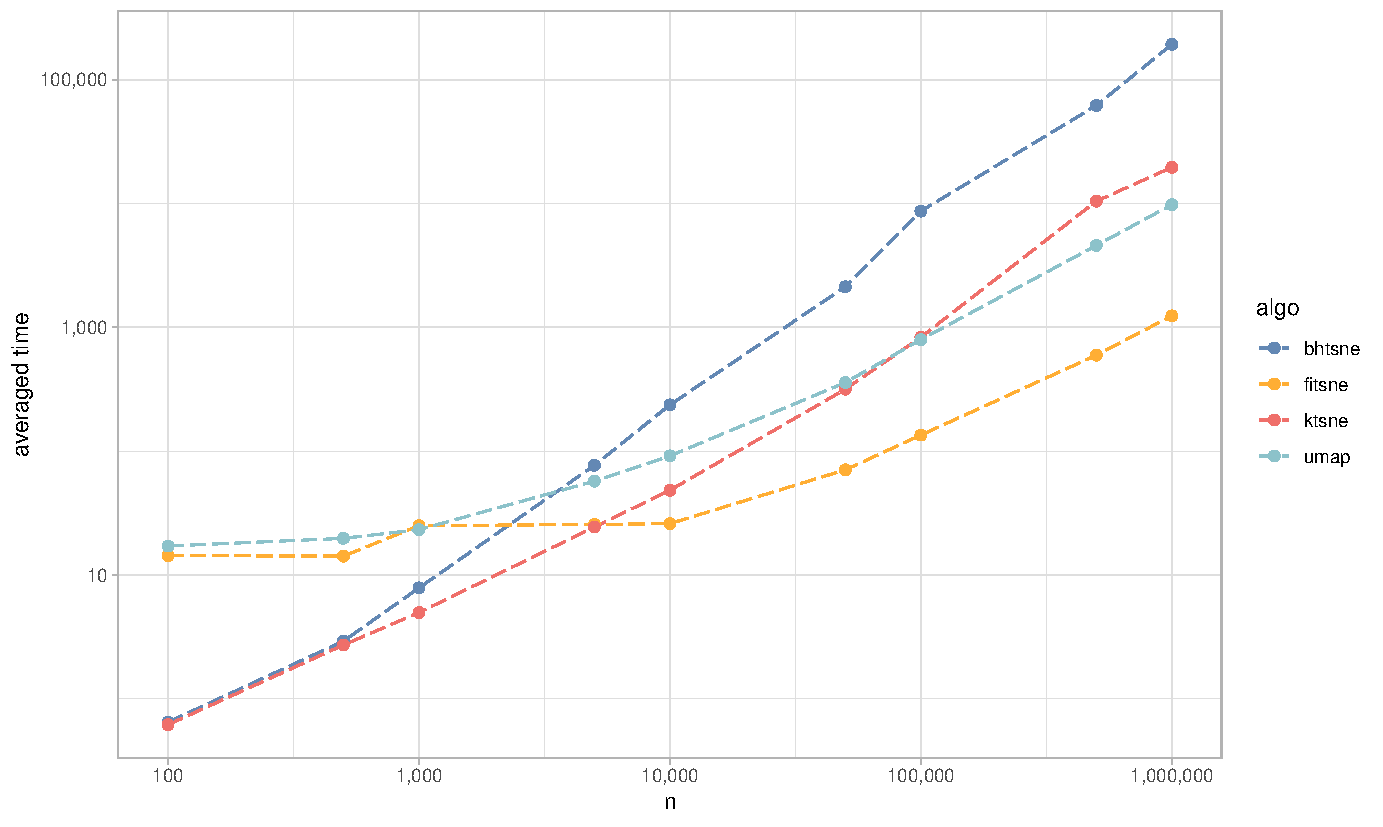
\includegraphics[width=0.9\textwidth]{runtime_comparison}
  \caption{Average runtime in seconds on synthetic data}
  \end{figure}
\end{frame}

\subsection{Some Embeddings}

\section{Conclusion}

\subsection{Summary}

\subsection{Future Work}

\begin{frame}[standout]
    Thanks for your attention!\\
    Any questions?
\end{frame}

\end{document}
